\documentclass[twocolumn,10pt]{article}
\usepackage[letterpaper,left=1.95cm,right=1.95cm,top=2.5cm,bottom=3.16cm]{geometry}
\usepackage{hyperref}
\usepackage{enumitem}
\usepackage{balance}
\usepackage{booktabs}
\usepackage{graphicx}
\usepackage{amsmath}
\usepackage{amssymb}
\graphicspath{{images/}}
\usepackage[utf8]{inputenc}
\usepackage{wasysym} % symbols
\usepackage{amssymb} % symbols
\usepackage{abstract}
\usepackage{parskip}
\usepackage{hyperref}
\usepackage{titlesec}
\usepackage{xcolor}
\usepackage{natbib}
\usepackage{float}
\usepackage{graphicx}
\usepackage{fancyhdr}
\usepackage{titling}
\usepackage{caption}
\usepackage[document]{ragged2e}
\usepackage[affil-sl]{authblk} 
\usepackage{mathptmx}  %Times new Roman

\setlength{\columnsep}{1cm}
\renewcommand{\refname}{BIBLIOGRAFÍA}
\renewcommand{\figurename}{Fig.}
\renewcommand{\tablename}{Tabla.}
\renewcommand{\abstractname}{RESUMEN}

% Keywords command
\providecommand{\keywordsSpan}[1]
{
  \small	
  \textbf{\textit{Palabras Clave:}} #1
}

\providecommand{\keywordsEng}[1]
{
  \small	
  \textbf{\textit{Keywords:}} #1
}


%%%%%%%% FORMATO DE LAS SECCIONES Y SUBSECCIONES %%%%%
\titleformat{\section} 
	{\normalfont\large\bfseries}{\makebox[30pt][l]{\thesection}}{0pt}{} 
\titleformat{\subsection} 
	{\normalfont\large\bfseries }{\makebox[30pt][l]{\thesubsection}}{0pt}{}
\renewcommand\thesection{\arabic{section}.}
\renewcommand\thesubsection{\thesection\arabic{subsection}}
%%%%%%%% FORMATO DE LAS SECCIONES Y SUBSECCIONES %%%%%


	
\makeatletter
\long\def\@makecaption#1#2{
\vskip\abovecaptionskip
\sbox\@tempboxa{#1. #2}
\ifdim \wd\@tempboxa >\hsize
#1. #2\par
\else
\global \@minipagefalse
\hb@xt@\hsize{\hfil\box\@tempboxa\hfil}
\fi
\vskip\belowcaptionskip}
\makeatother


\pagestyle{fancyplain}% <- pagestyle fancyplain

\fancyfoot[C]{}
\renewcommand\plainheadrulewidth{.4pt}% headrule on plain pages
%\fancyhf{}
\rhead{Semestre 4 Año 2026}
\lhead{Estadística Bayesiana}
\rfoot{\thepage}

\date{}
 

%%%%%%% ENCABEZADO %%%%%%%%%%%%%%%%%%%%

{\title{\fontsize{16}{16}\selectfont
\vspace*{-0.7cm}
\textbf{
¿Qué hace que un equipo gane? Un análisis bayesiano sobre la victoria en CS:GO
} \\[0.2cm]
\fontsize{12}{12}\selectfont
\textbf{Predicting the Unpredictable: Descubriendo las Variables más Influyentes en la Victoria y Cuantificando la Incertidumbre en el Servidor}\\[0.2cm]}
}

\author[1,*]{\fontsize{10pt}{10pt}\selectfont \textbf{Julián Duarte}}
\author[2]{\textbf{Julián Jiménez}}
\author[3]{\textbf{Tomás Rincón}}

\affil[1]{\fontsize{8pt}{8pt}\selectfont Pregrado Ciencia de Datos Universidad Externado, Bogotá - Colombia}
\affil[2]{Pregrado Ciencia de Datos Universidad Externado, Bogotá - Colombia}
\affil[3]{Pregrado Ciencia de Datos Universidad Externado, Bogotá - Colombia \vspace{0.2cm}} 
\affil[*]{julian.duarte2@est.uexternado.edu.co; julian.jimenez5@est.uexternado.edu.co; juan.rincon14@est.uexternado.edu.co}

\begin{document}

\twocolumn[
  \begin{@twocolumnfalse}
    \maketitle

    \begin{center}
        \textbf{RESUMEN}
    \end{center}
    Este proyecto nace de la curiosidad por entender cómo se gana realmente en el mundo profesional del Counter-Strike. Mediante un enfoque bayesiano, se analizan miles de partidas de alto nivel para encontrar qué variables son las que de verdad inclinan la balanza. A diferencia de los modelos comunes que solo dan un porcentaje fijo, esta investigación se enfoca en medir la incertidumbre para saber qué tan confiable es cada predicción. Los resultados muestran que al usar información previa y considerar la diferencia entre mapas, se logra una visión más realista de las probabilidades de éxito\cite{csgodataset2020}.
    \vspace{0.2cm}

    \keywordsSpan{Esports, Modelado Bayesiano, CS:GO, Análisis de Datos, Incertidumbre, Validación Predictiva.}
    
    \vspace{0.6cm}
  \end{@twocolumnfalse}
]

\thispagestyle{fancyplain}

\section{PLANTEAMIENTO DEL PROBLEMA}
Imagina que se está viendo la Gran Final de un Mundial de CS:GO. El marcador está 14-14 en el mapa de \textit{Inferno} y la tensión se siente en cada segundo del reloj. De repente, el jugador estrella del equipo hace una jugada increíble: tres bajas seguidas que dejan a todos gritando. Sus números suben y parece que tienen la ronda ganada. Pero, en un parpadeo, el otro equipo logra desactivar la bomba y se lleva el mapa. Aquí es donde surge la duda que motiva este proyecto: ¿por qué si un jugador brilla tanto, su equipo termina perdiendo? Muchas veces las variables que se observan en pantalla solo cuentan una parte de la historia y no explican realmente qué es lo que hace que un equipo gane en medio de tanto caos.

El problema es que la mayoría de los modelos de predicción que existen nos dan un número fijo, como si ganar fuera algo seguro, y se olvidan de que en el Counter-Strike el azar y el contexto del mapa cambian todo. A esto se le conoce como \textbf{incertidumbre epistémica}, pero en palabras simples, es reconocer que hay muchas cosas que no podemos predecir con total seguridad. El reto de este trabajo no es solo adivinar quién va a ganar, sino entender qué tan confiable es esa predicción cuando el juego es tan volátil. Queremos descubrir cuáles son las variables más influyentes que actúan como motores de la victoria cuando la competencia está tan pareja.

\section{PREGUNTA DE INVESTIGACIÓN Y OBJETIVOS}

Para resolver este misterio y no caer en el error de dar números fijos que ignoran el azar, se decidió usar un enfoque que permita ser ``honestos'' con lo que no se sabe. Es aquí donde el modelado bayesiano se vuelve el mejor aliado, llevando a la siguiente duda:

\subsection{Pregunta de Investigación}
¿Cuáles son las variables que se posicionan como los determinantes más influyentes de la victoria en CS:GO y de qué manera este enfoque bayesiano ayuda a cuantificar la incertidumbre de los pronósticos ante la volatilidad del escenario profesional?

\subsection{Objetivos}
\textbf{Objetivo General:}
Identificar cuáles son las variables que actúan como los determinantes más influyentes de la victoria y desarrollar un modelo bayesiano que permita estimar las probabilidades de éxito, midiendo siempre la incertidumbre de las predicciones en el circuito profesional de CS:GO.

\textbf{Objetivos Específicos:}
\begin{itemize}
    \item Explorar miles de partidas profesionales para encontrar las variables que realmente separan a los ganadores de los perdedores.
    \item Integrar lo que ya se conoce sobre el desempeño de los equipos (\textit{priors}) para que el modelo sea más confiable frente a resultados inesperados.
    \item Implementar un sistema que no solo nos arroje un ganador, sino que nos permita visualizar qué tan seguros estamos de ese pronóstico.
    \item Evaluar el desempeño del modelo mediante Chequeos Predictivos Posteriores (PPC) y el análisis de los intervalos HDI.
\end{itemize}

\section{JUSTIFICACIÓN}
Este proyecto se realiza porque se considera que en los Esports faltan análisis que sean honestos con lo impredecible que es el juego. Muchas veces se observa solo el resultado final, pero no se entiende qué tan arriesgado fue llegar ahí. El modelado bayesiano da esa herramienta para unir los datos con la realidad del servidor, permitiendo que analistas y aficionados entiendan no solo quién tiene más chance de ganar, sino cuánta duda hay detrás de ese número\cite{sainz2024bayesian}.

\section{ESTADO DEL ARTE}
Para hacer este proyecto, investigamos lo que otros ya han hecho y nos dimos cuenta de que el análisis de datos en los Esports ha avanzado un montón. Por ejemplo, autores como Broms y Nordansj\"{o}\cite{csgodataset2020} o Makarov\cite{makarov2017predicting} han usado modelos de aprendizaje automático para intentar adivinar quién gana las partidas. También vimos que existen sistemas muy conocidos como el \textit{TrueSkill} de Microsoft\cite{herbrich2006trueskill}, que usa ideas bayesianas para ponerles puntaje a los jugadores, y otros estudios que miran cómo cambian las probabilidades de ganar mientras se juega la partida\cite{hodge2019win}.

A pesar de todo esto, sentimos que a muchos de estos modelos les falta algo: la capacidad de decirte qué tan seguros están de su predicción. Como menciona Goldin\cite{goldin2021bayesian}, el CS:GO cambia constantemente y no se puede tratar cada partida como algo aislado. Por eso, nosotros decidimos ir un paso más allá. Usando las bases de expertos en estadística como Gelman\cite{gelman2013bayesian}, diseñamos un modelo que no solo busca al ganador, sino que mide la incertidumbre. Así, nuestro trabajo no solo intenta predecir, sino que es lo suficientemente ``honesto'' para reconocer cuándo un resultado es demasiado difícil de asegurar debido a lo volátil que es el juego.

\section{CONTEXTO DEL PROBLEMA}
Hoy en día, el Counter-Strike es una industria gigante que mueve millones de dólares y atrae a más de un millón y medio de personas en las finales. Todo este crecimiento ha hecho que se generen muchísimos datos, y páginas como \textit{HLTV.org} guardan los datos de miles de partidas cada año. 

Ahora mismo, el nivel de los equipos es tan parecido que la diferencia entre ganar y perder es mínima. Cosas como qué tan bien juega un equipo en un mapa específico o cómo rinden bajo presión son claves. Por eso, necesitamos herramientas que entiendan que una ventaja puede desaparecer en un segundo y que el éxito depende de qué tan bien se adapte un equipo a lo que pasa en la partida.

\section{FUENTE DE DATOS Y VARIABLES}
Para que nuestro estudio tenga bases sólidas, usamos una base de datos con más de 3,700 partidas profesionales. Aquí te mostramos las variables clave que usamos como las piezas principales para armar nuestro modelo:

\begin{table}[!ht]
\centering
\caption{Diccionario de Variables.}
\label{tab:data_dict}
\begin{tabular}{lp{5.2cm}}
\toprule
\textbf{Variable} & \textbf{Definición} \\
\midrule
\textbf{Rating 2.0} & Variable integral de rendimiento (Kills, Supervivencia, Impacto). \\
\textbf{ADR} & Promedio de daño infligido por ronda. \\
\textbf{Impacto} & Peso en momentos críticos (multikills y \textit{opening kills}). \\
\textbf{KAST} & \% de rondas con contribución directa (Baja, Asistencia, Supervivencia). \\
\textbf{Winrate} & Tasa de victorias histórica en el mapa seleccionado. \\
\bottomrule
\end{tabular}
\end{table}

\section{ANÁLISIS EXPLORATORIO DE DATOS (EDA)}
Se analizan a fondo los datos de las partidas para identificar los factores y variables que actúan como los verdaderos motores del éxito competitivo, justificando la estructura del modelo propuesto.

\subsection{Análisis de Paridad y Distribución}
En la Figura \ref{fig:DistFig} se observa una superposición extrema en las distribuciones de \textit{Rating} entre los equipos de élite. Esta paridad técnica confirma que el nivel competitivo es tan cercano que un simple ranking no es suficiente para predecir un ganador. Es precisamente este hallazgo el que justifica el uso de un enfoque bayesiano: ante la imposibilidad de discriminar a los equipos por talento puro, se vuelve vital cuantificar la \textbf{incertidumbre epistémica} para entender los márgenes de victoria.

\begin{figure}[h]
    \centering
    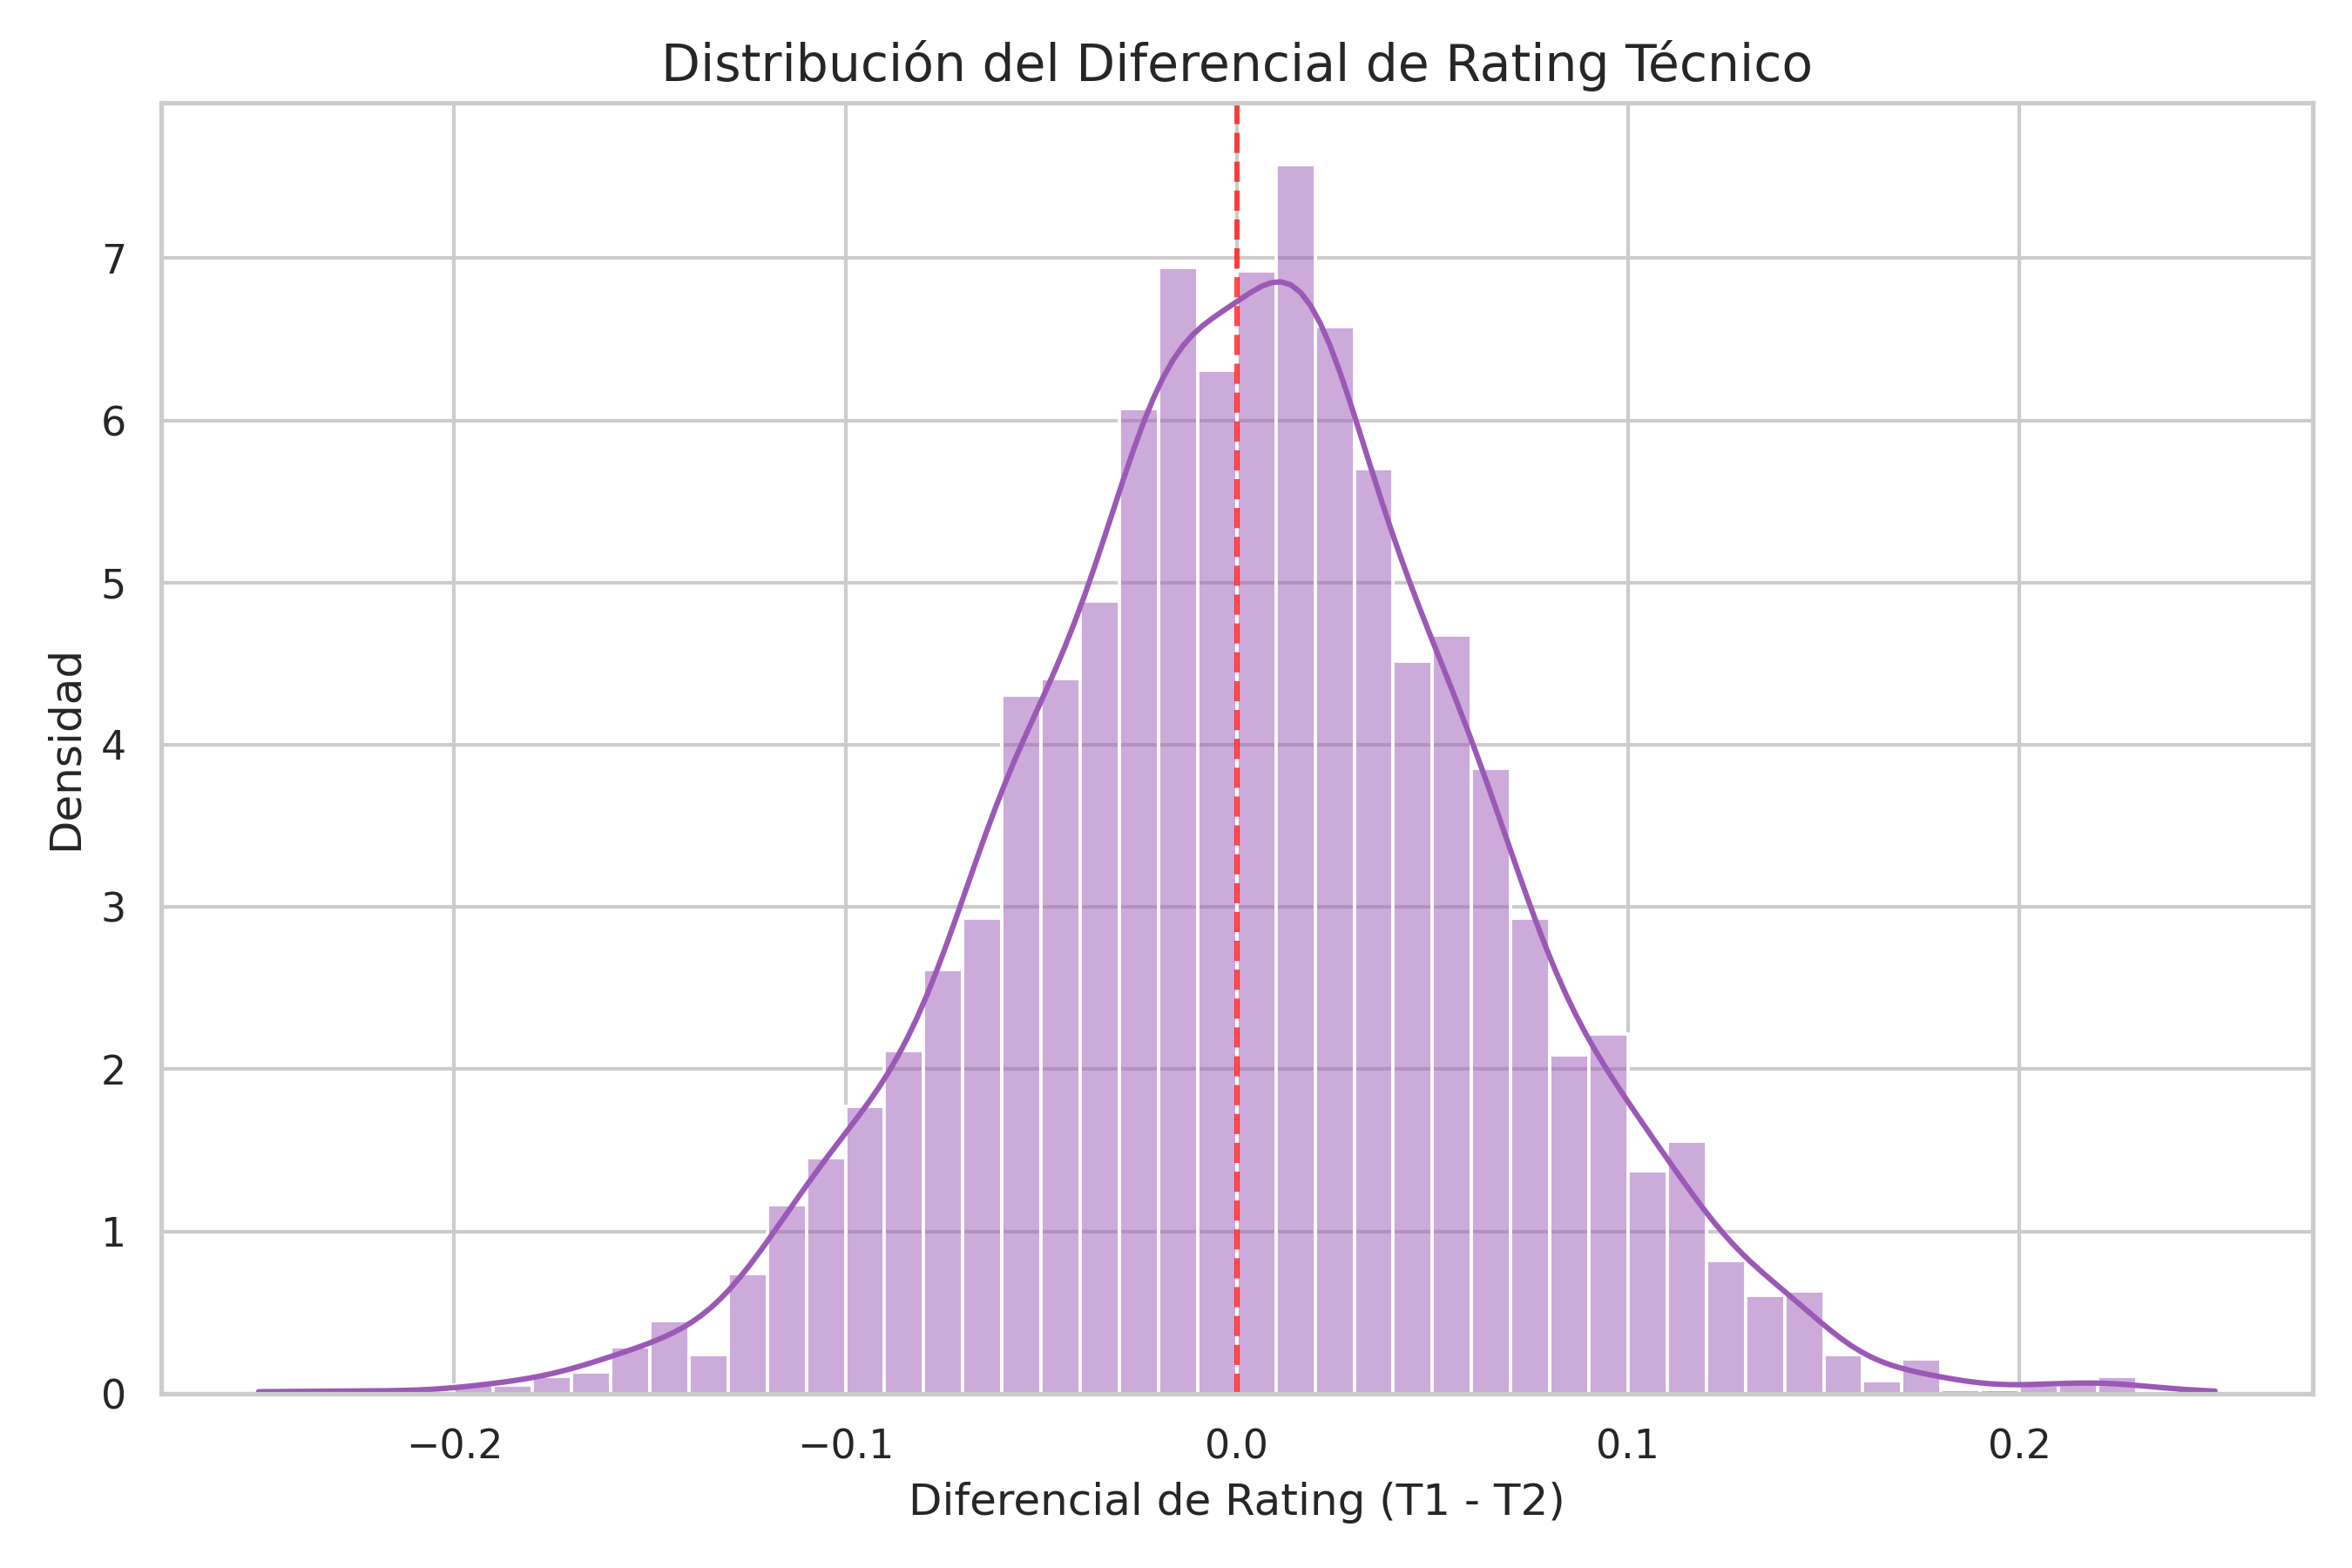
\includegraphics[width=\linewidth]{distribucion_densidad_rating.png}
    \caption{Distribución del Rating: La paridad extrema en la élite.}
    \label{fig:DistFig}
\end{figure}

\subsection{Relación entre Desempeño y Éxito}
La Figura \ref{fig:RatingWin} valida que las métricas de rendimiento individual se traducen efectivamente en éxitos colectivos. Se observa una correlación positiva donde incluso mejoras marginales en el desempeño promedio del equipo aumentan significativamente la probabilidad de victoria. Este análisis posiciona al \textit{Rating} como la variable base para iniciar la discriminación entre ganadores y perdedores.

\begin{figure}[h]
    \centering
    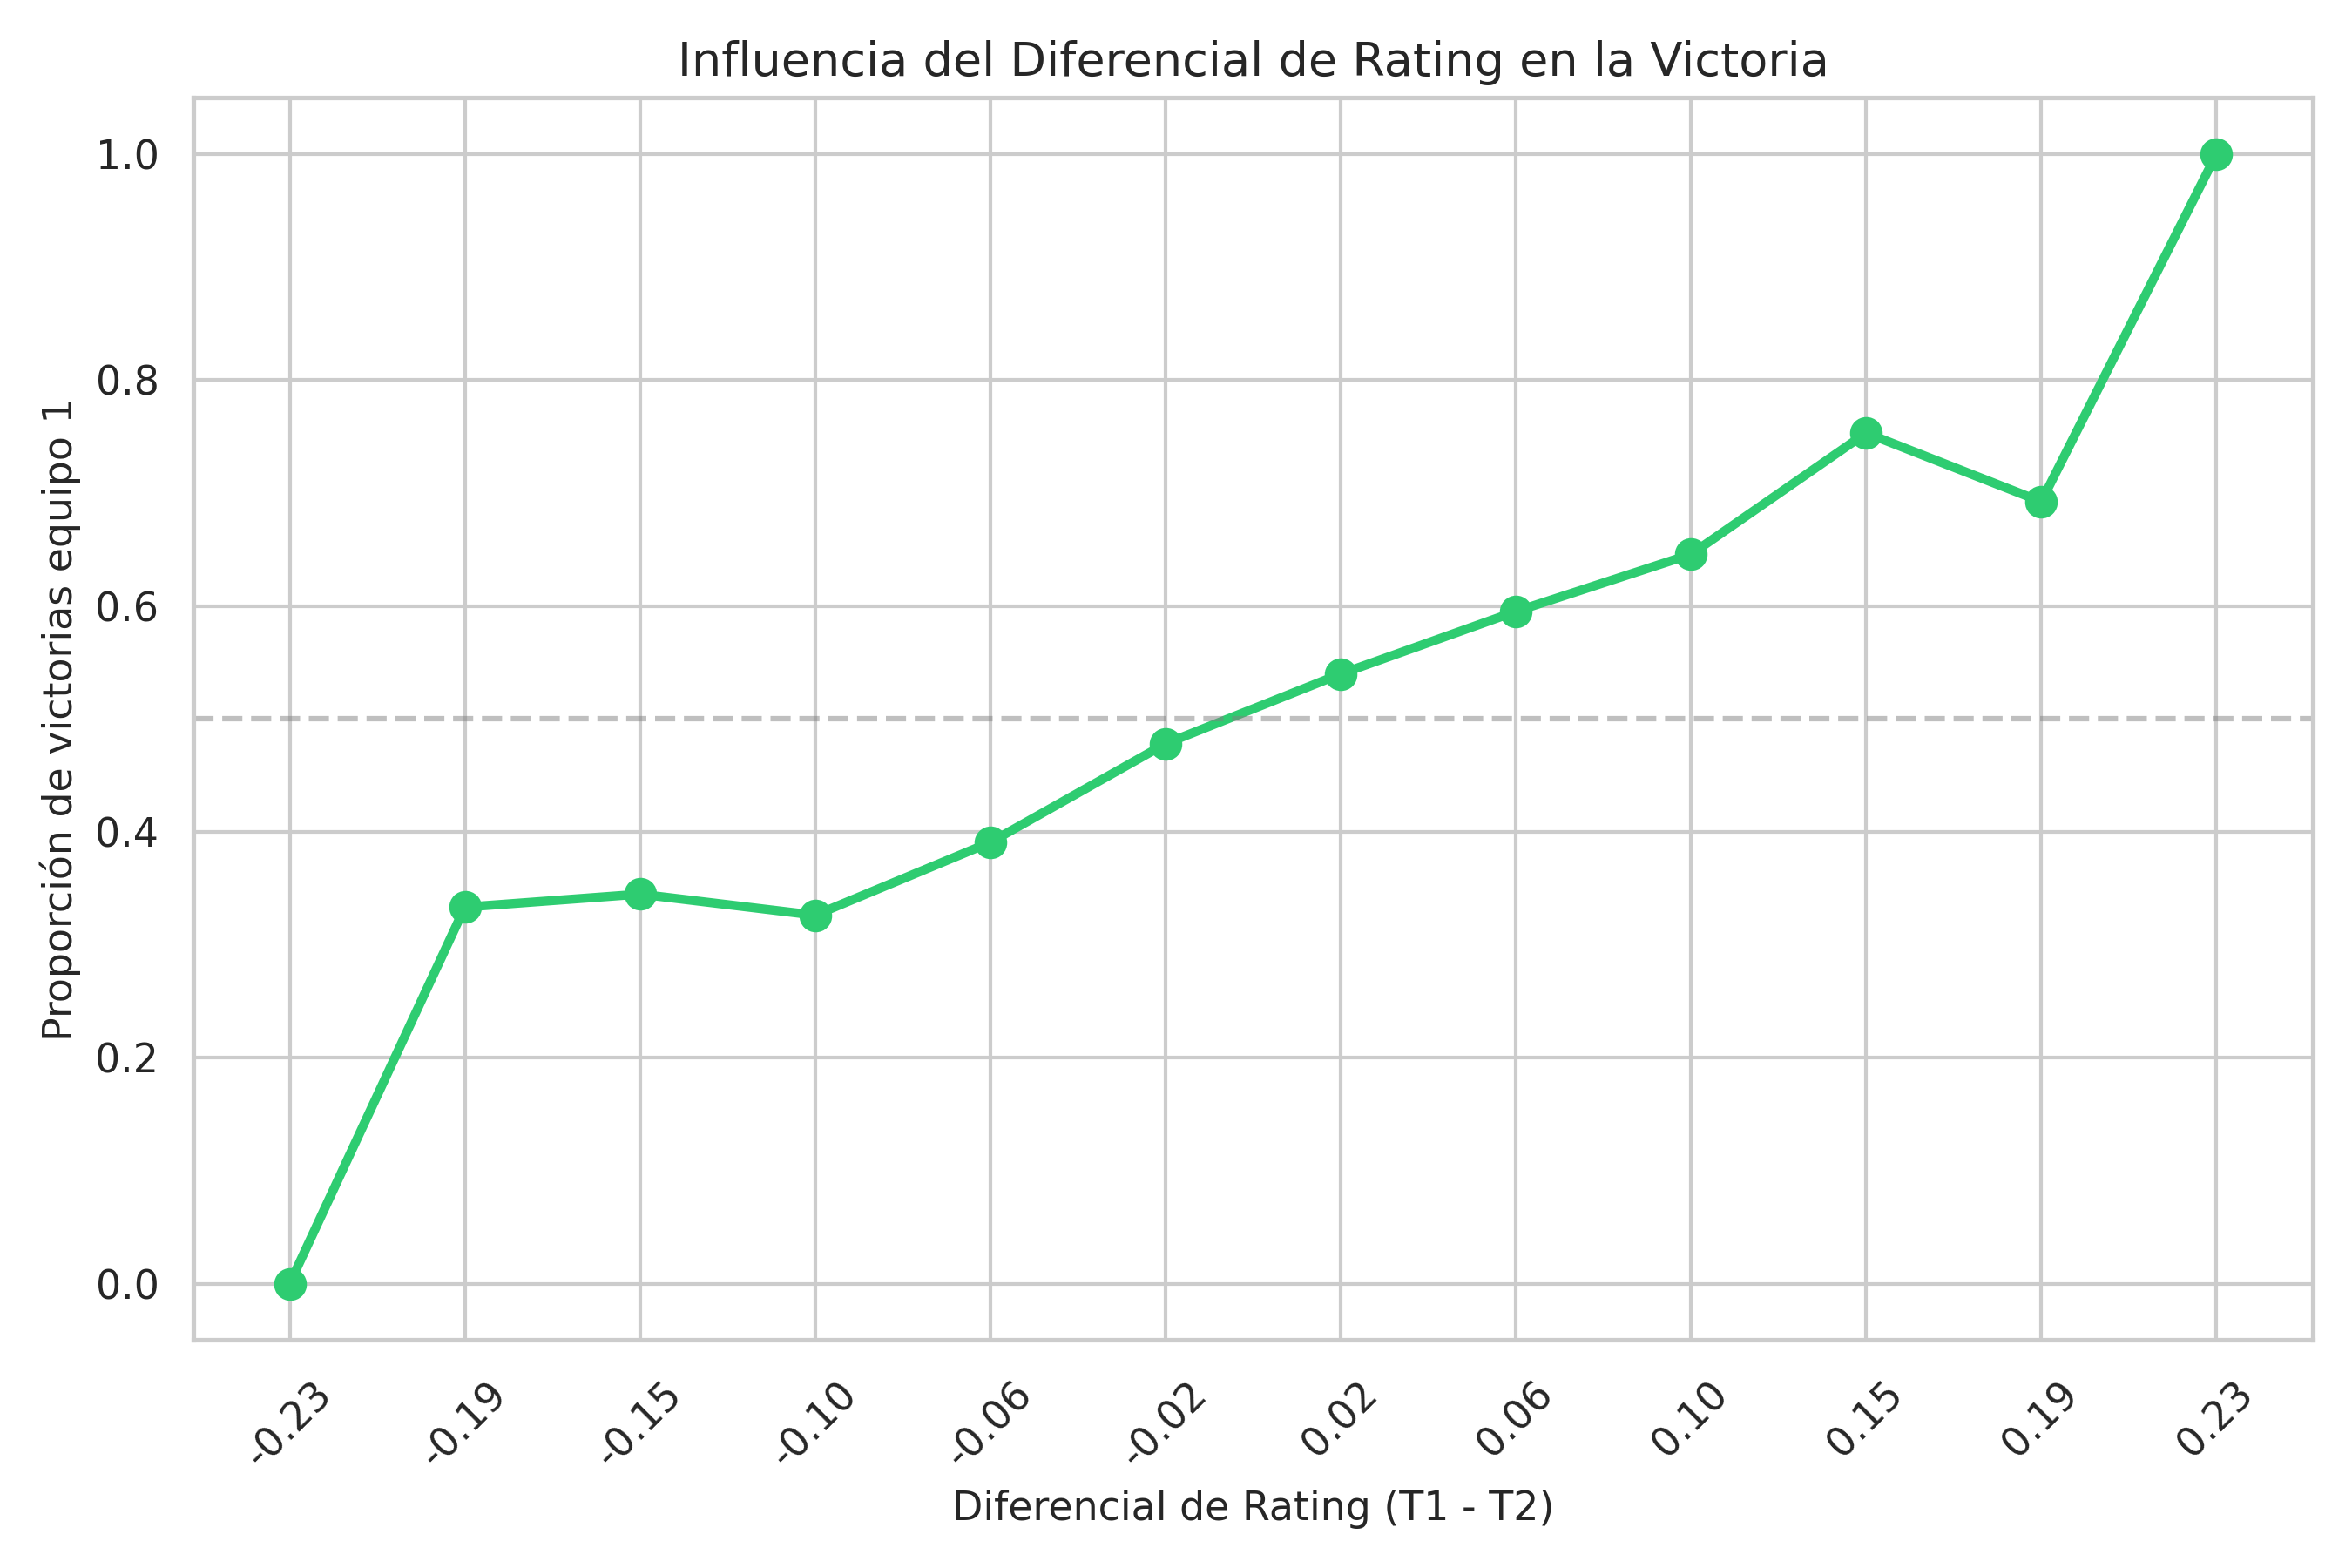
\includegraphics[width=\linewidth]{evidencia_rating_winrate.png}
    \caption{Evidencia Rating vs Winrate: El peso del talento.}
    \label{fig:RatingWin}
\end{figure}

\subsection{Motores de la Victoria: Impacto y Contexto Táctico}
Para entender por qué equipos con estadísticas similares obtienen resultados distintos, se analizó el \textbf{Impacto Táctico}. En la Figura \ref{fig:ImpactViolin} se aprecia que los ganadores poseen un impacto mucho más constante, lo que sugiere que el éxito no solo depende de la cantidad de bajas, sino de su relevancia en momentos críticos (como las \textit{opening kills}). 

Además, el balance de los mapas (Figura \ref{fig:MapBalance}) revela asimetrías tácticas significativas entre el bando defensivo (CT) y el ofensivo (T). Esta variabilidad contextual es la que motiva la implementación de una \textbf{estructura jerárquica} en el modelo, permitiendo que las predicciones se ajusten según las características únicas de cada escenario de juego.

\begin{figure}[h]
    \centering
    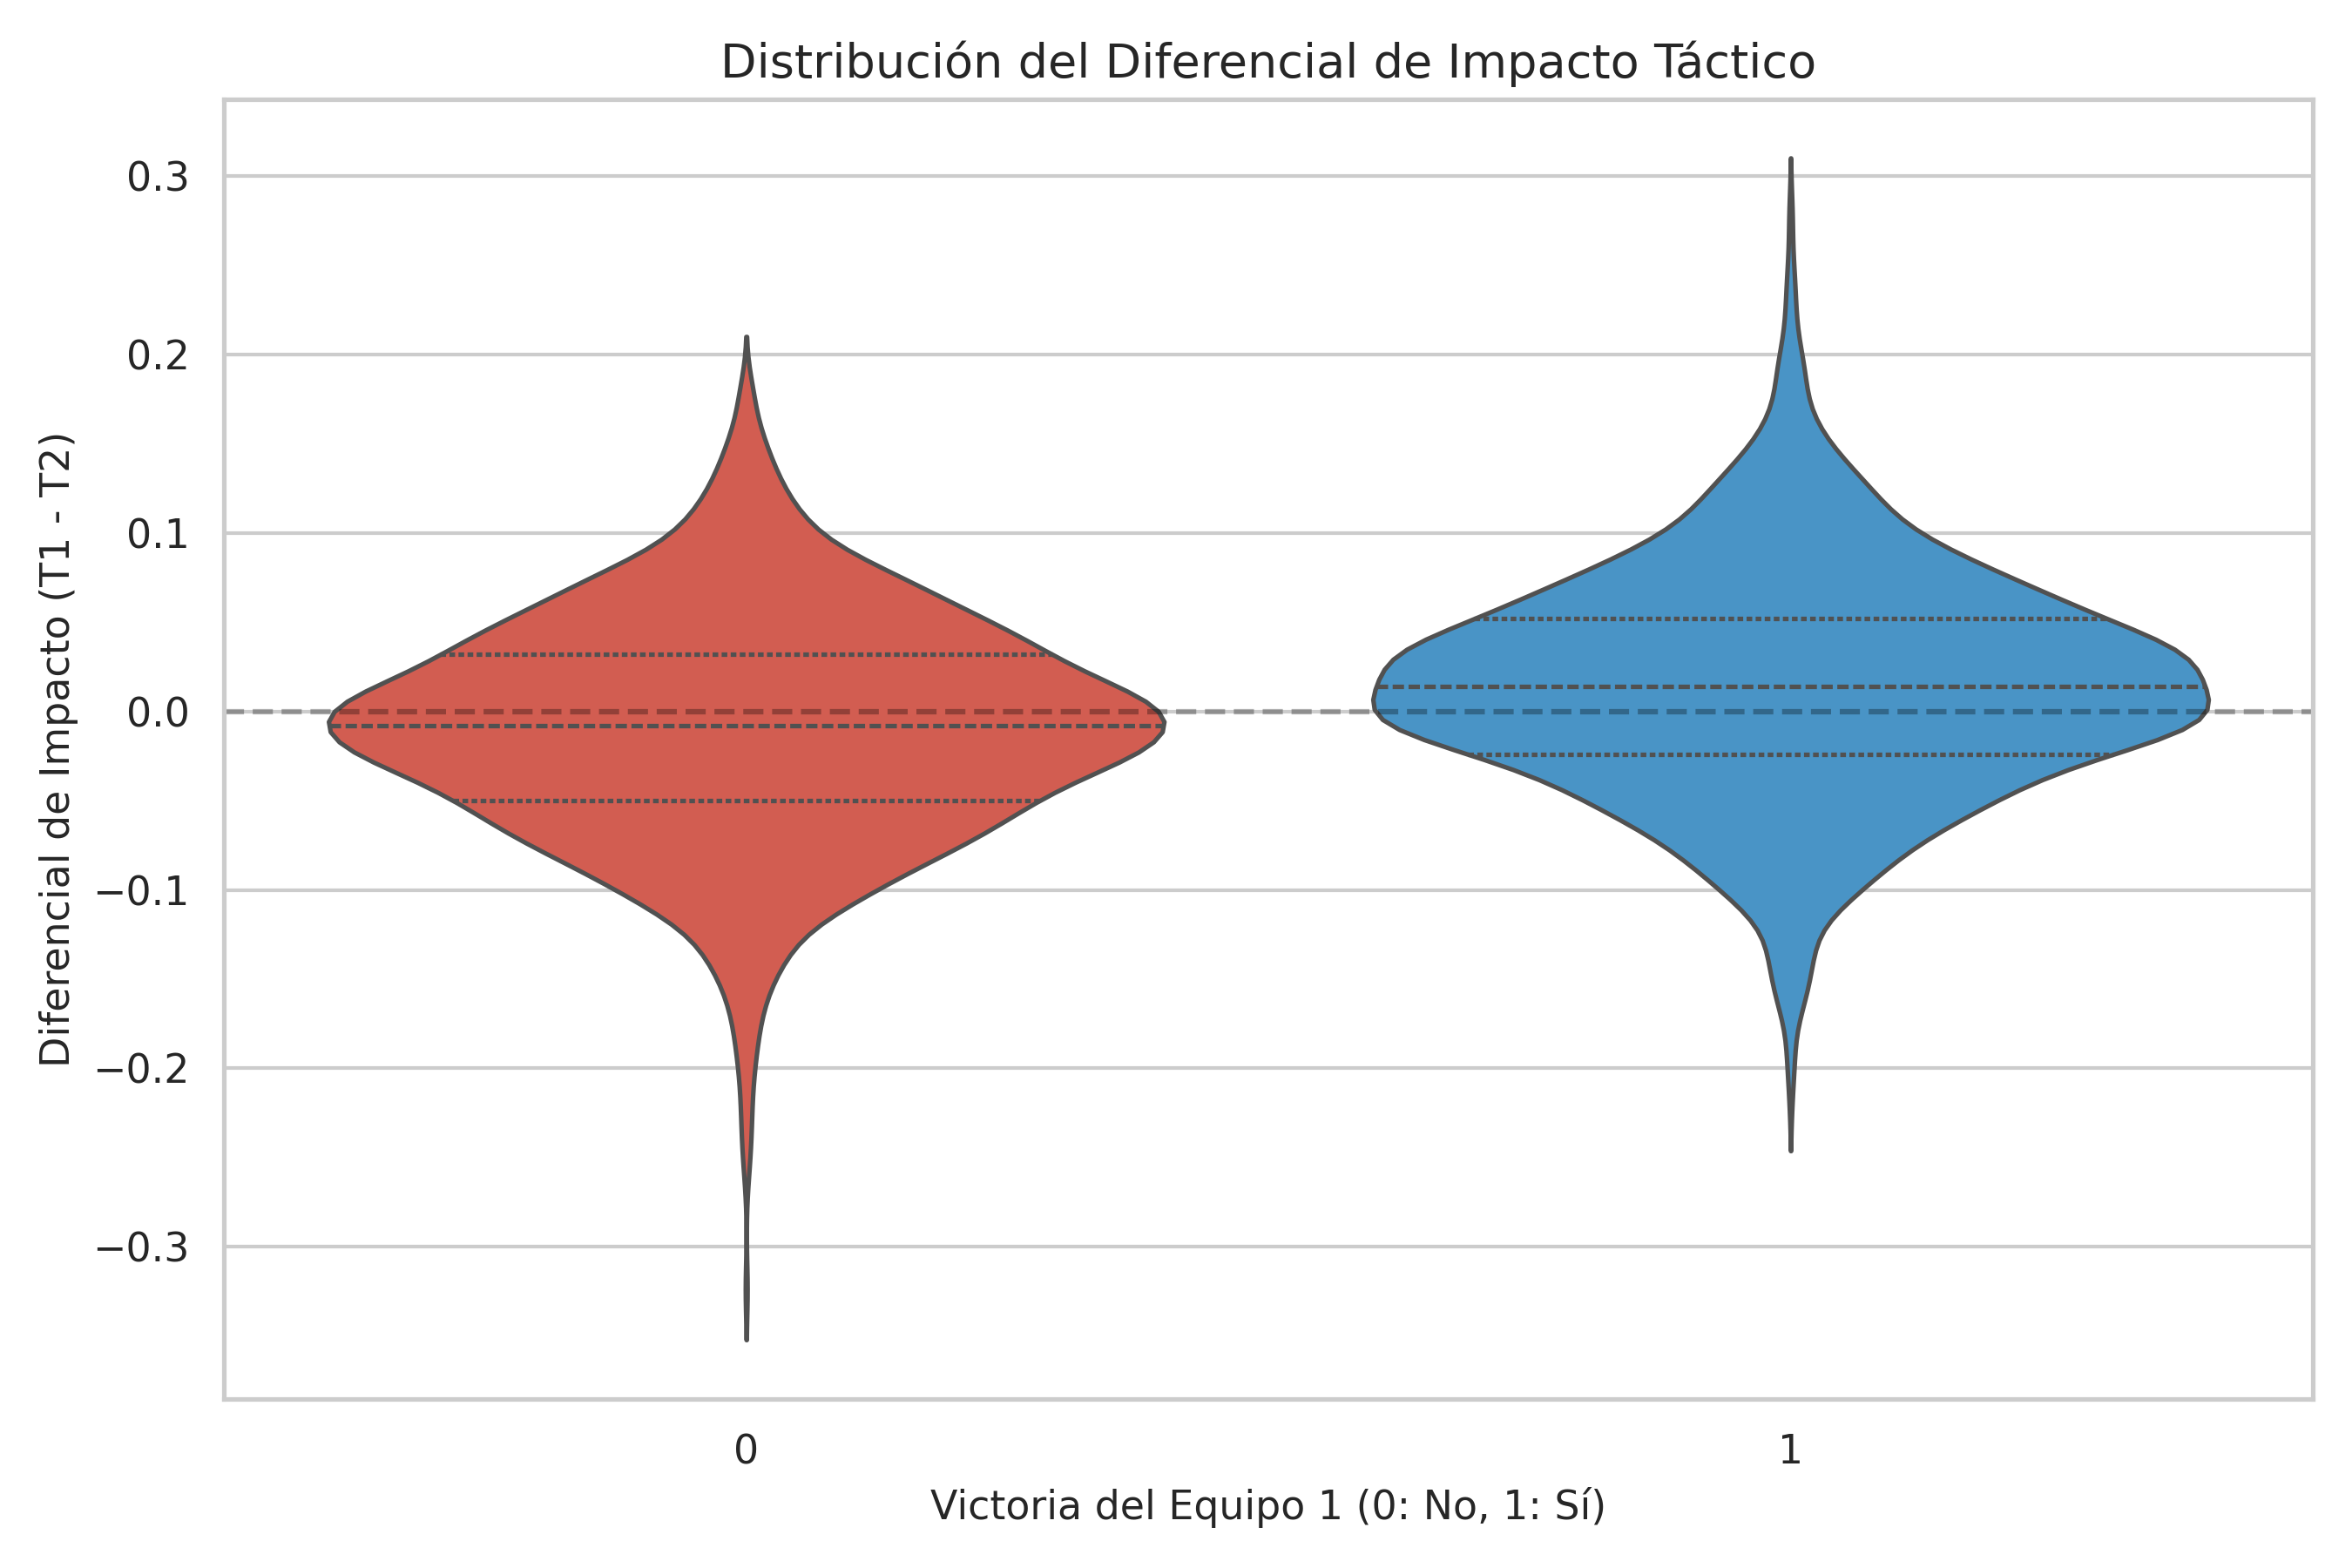
\includegraphics[width=\linewidth]{evidencia_impacto_violin.png}
    \caption{Análisis de Impacto: Comparativa de densidad.}
    \label{fig:ImpactViolin}
\end{figure}

\begin{figure}[h]
    \centering
    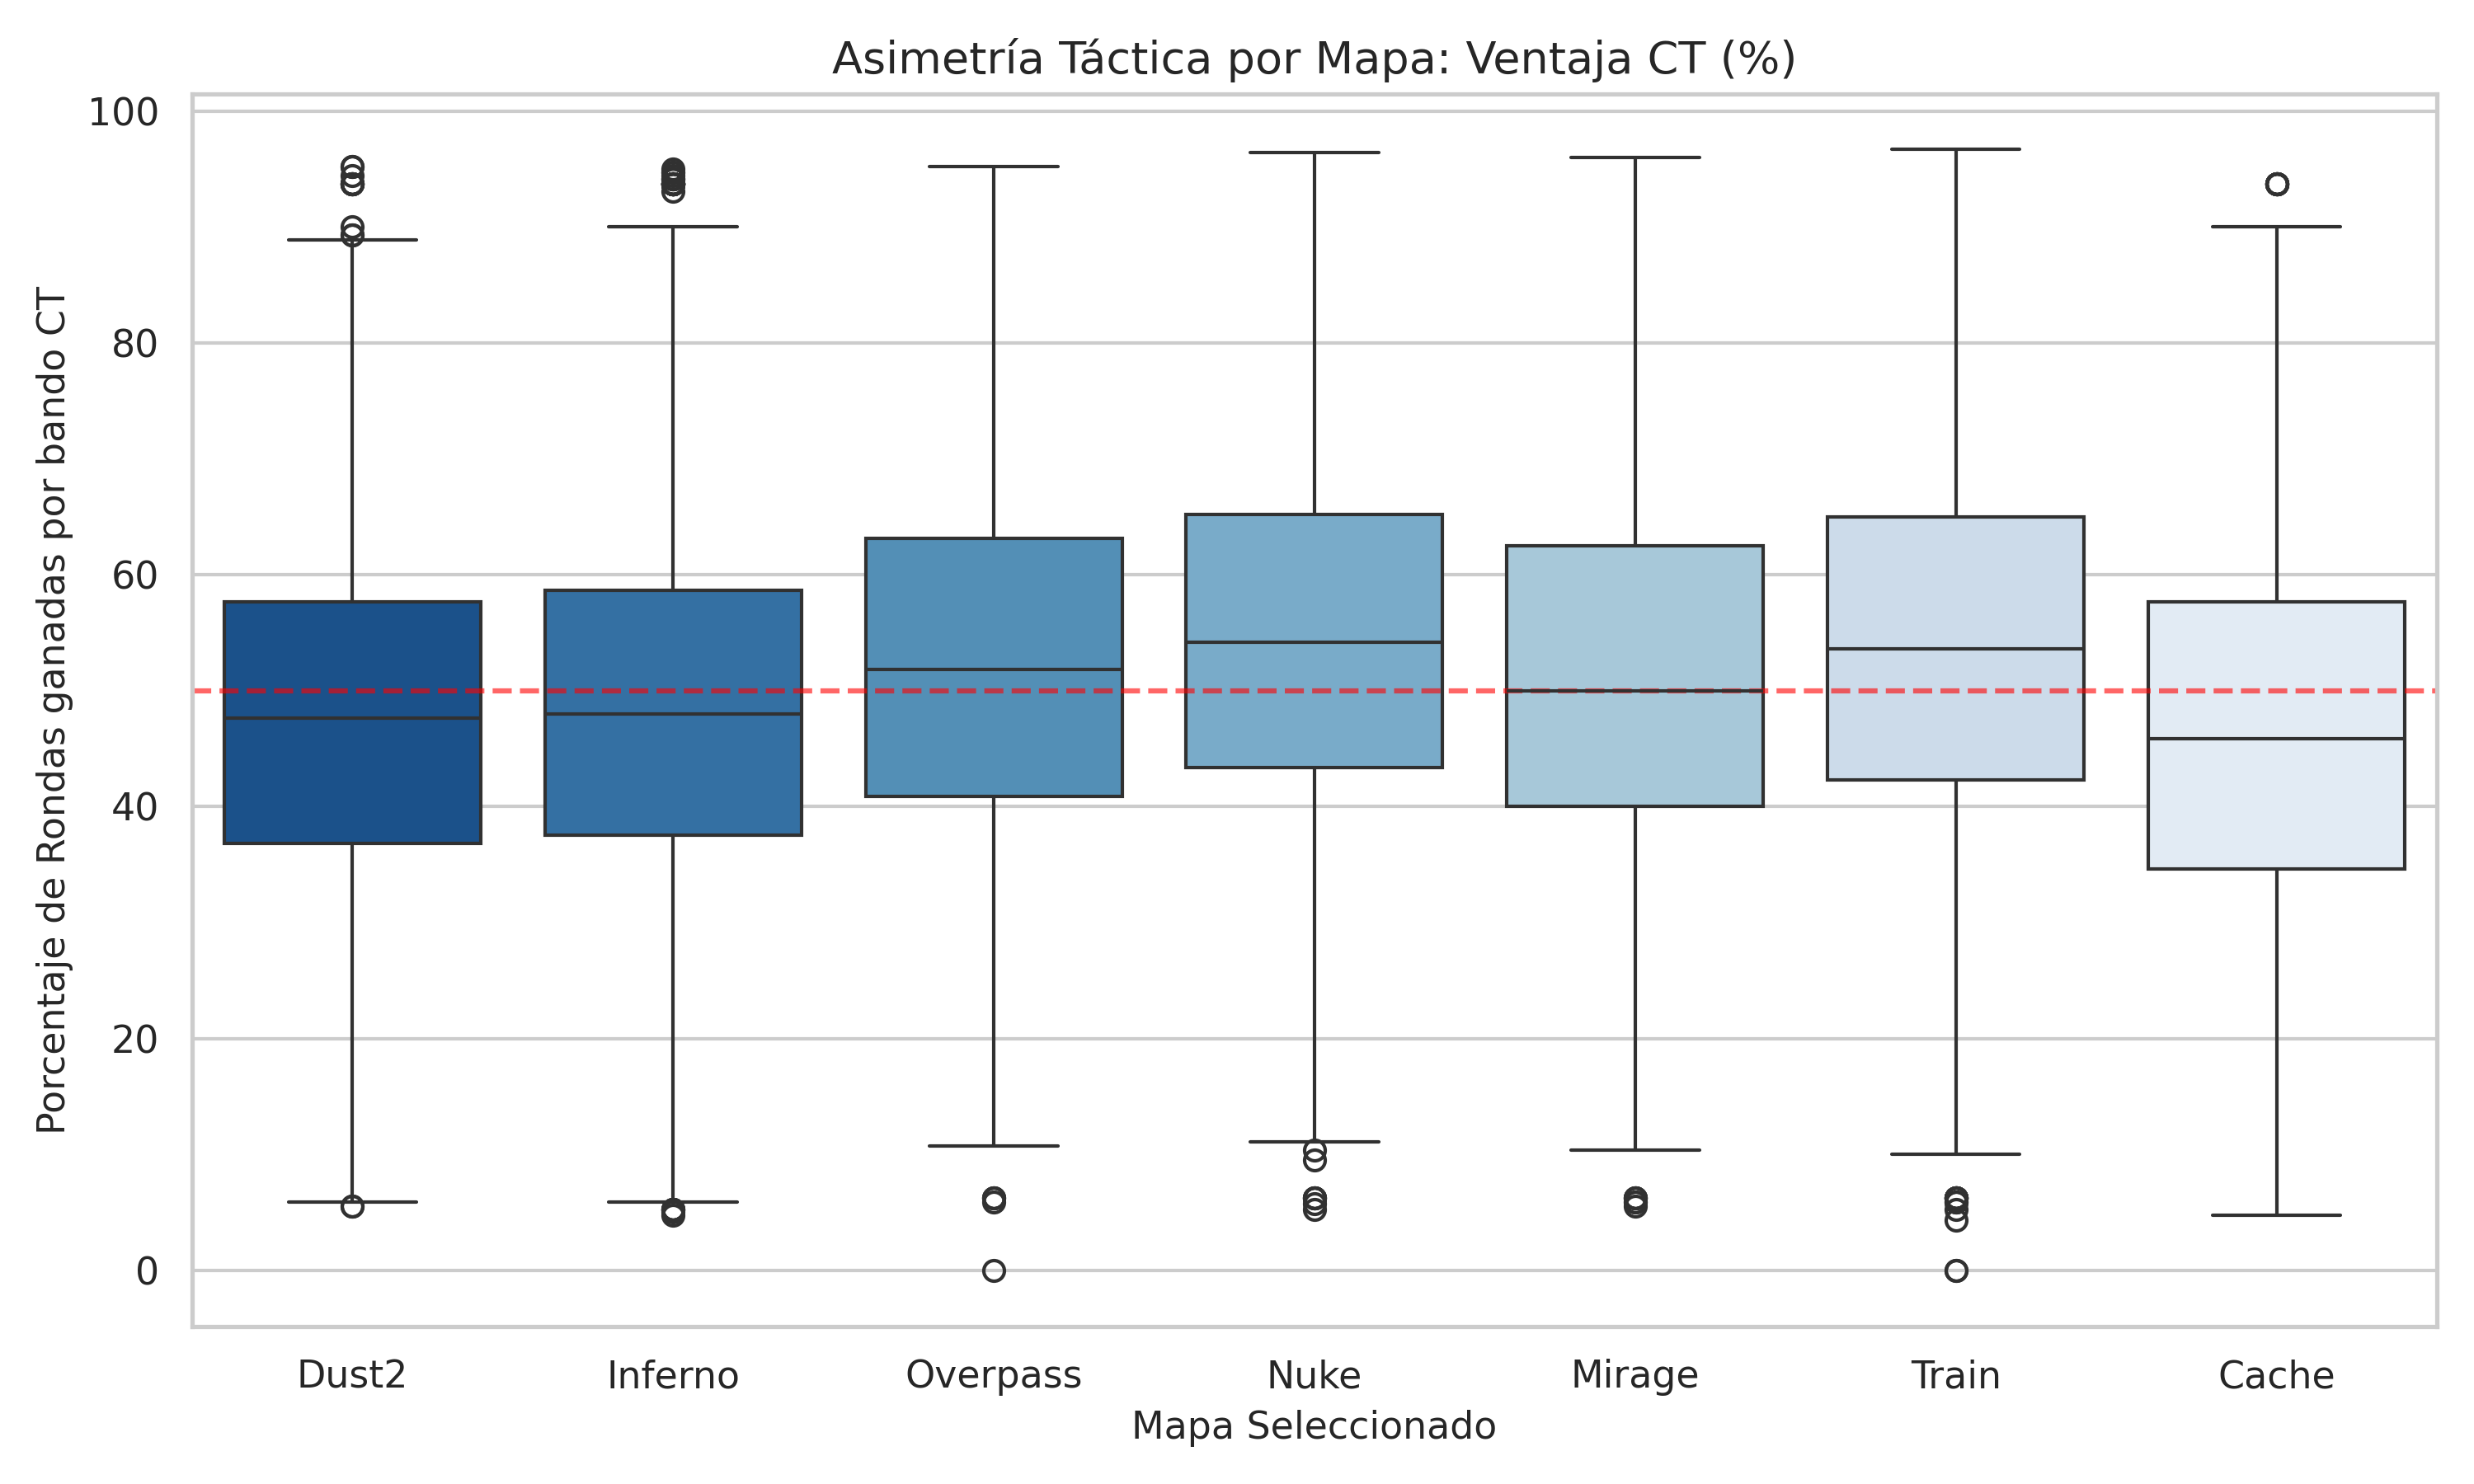
\includegraphics[width=\linewidth]{balance_ct_t_mapas.png}
    \caption{Balance CT/T: La asimetría táctica de los mapas.}
    \label{fig:MapBalance}
\end{figure}

\subsection{Matriz de Correlación}
Finalmente, la matriz de correlación (Figura \ref{fig:CorrFig}) identifica la sinergia fundamental entre el Impacto Táctico y el Daño Promedio (ADR). Estos hallazgos confirman que los verdaderos motores de la victoria son aquellas variables que capturan la capacidad de influir en el servidor en momentos de alta presión, formando el núcleo predictivo del estudio.

\begin{figure}[h]
    \centering
    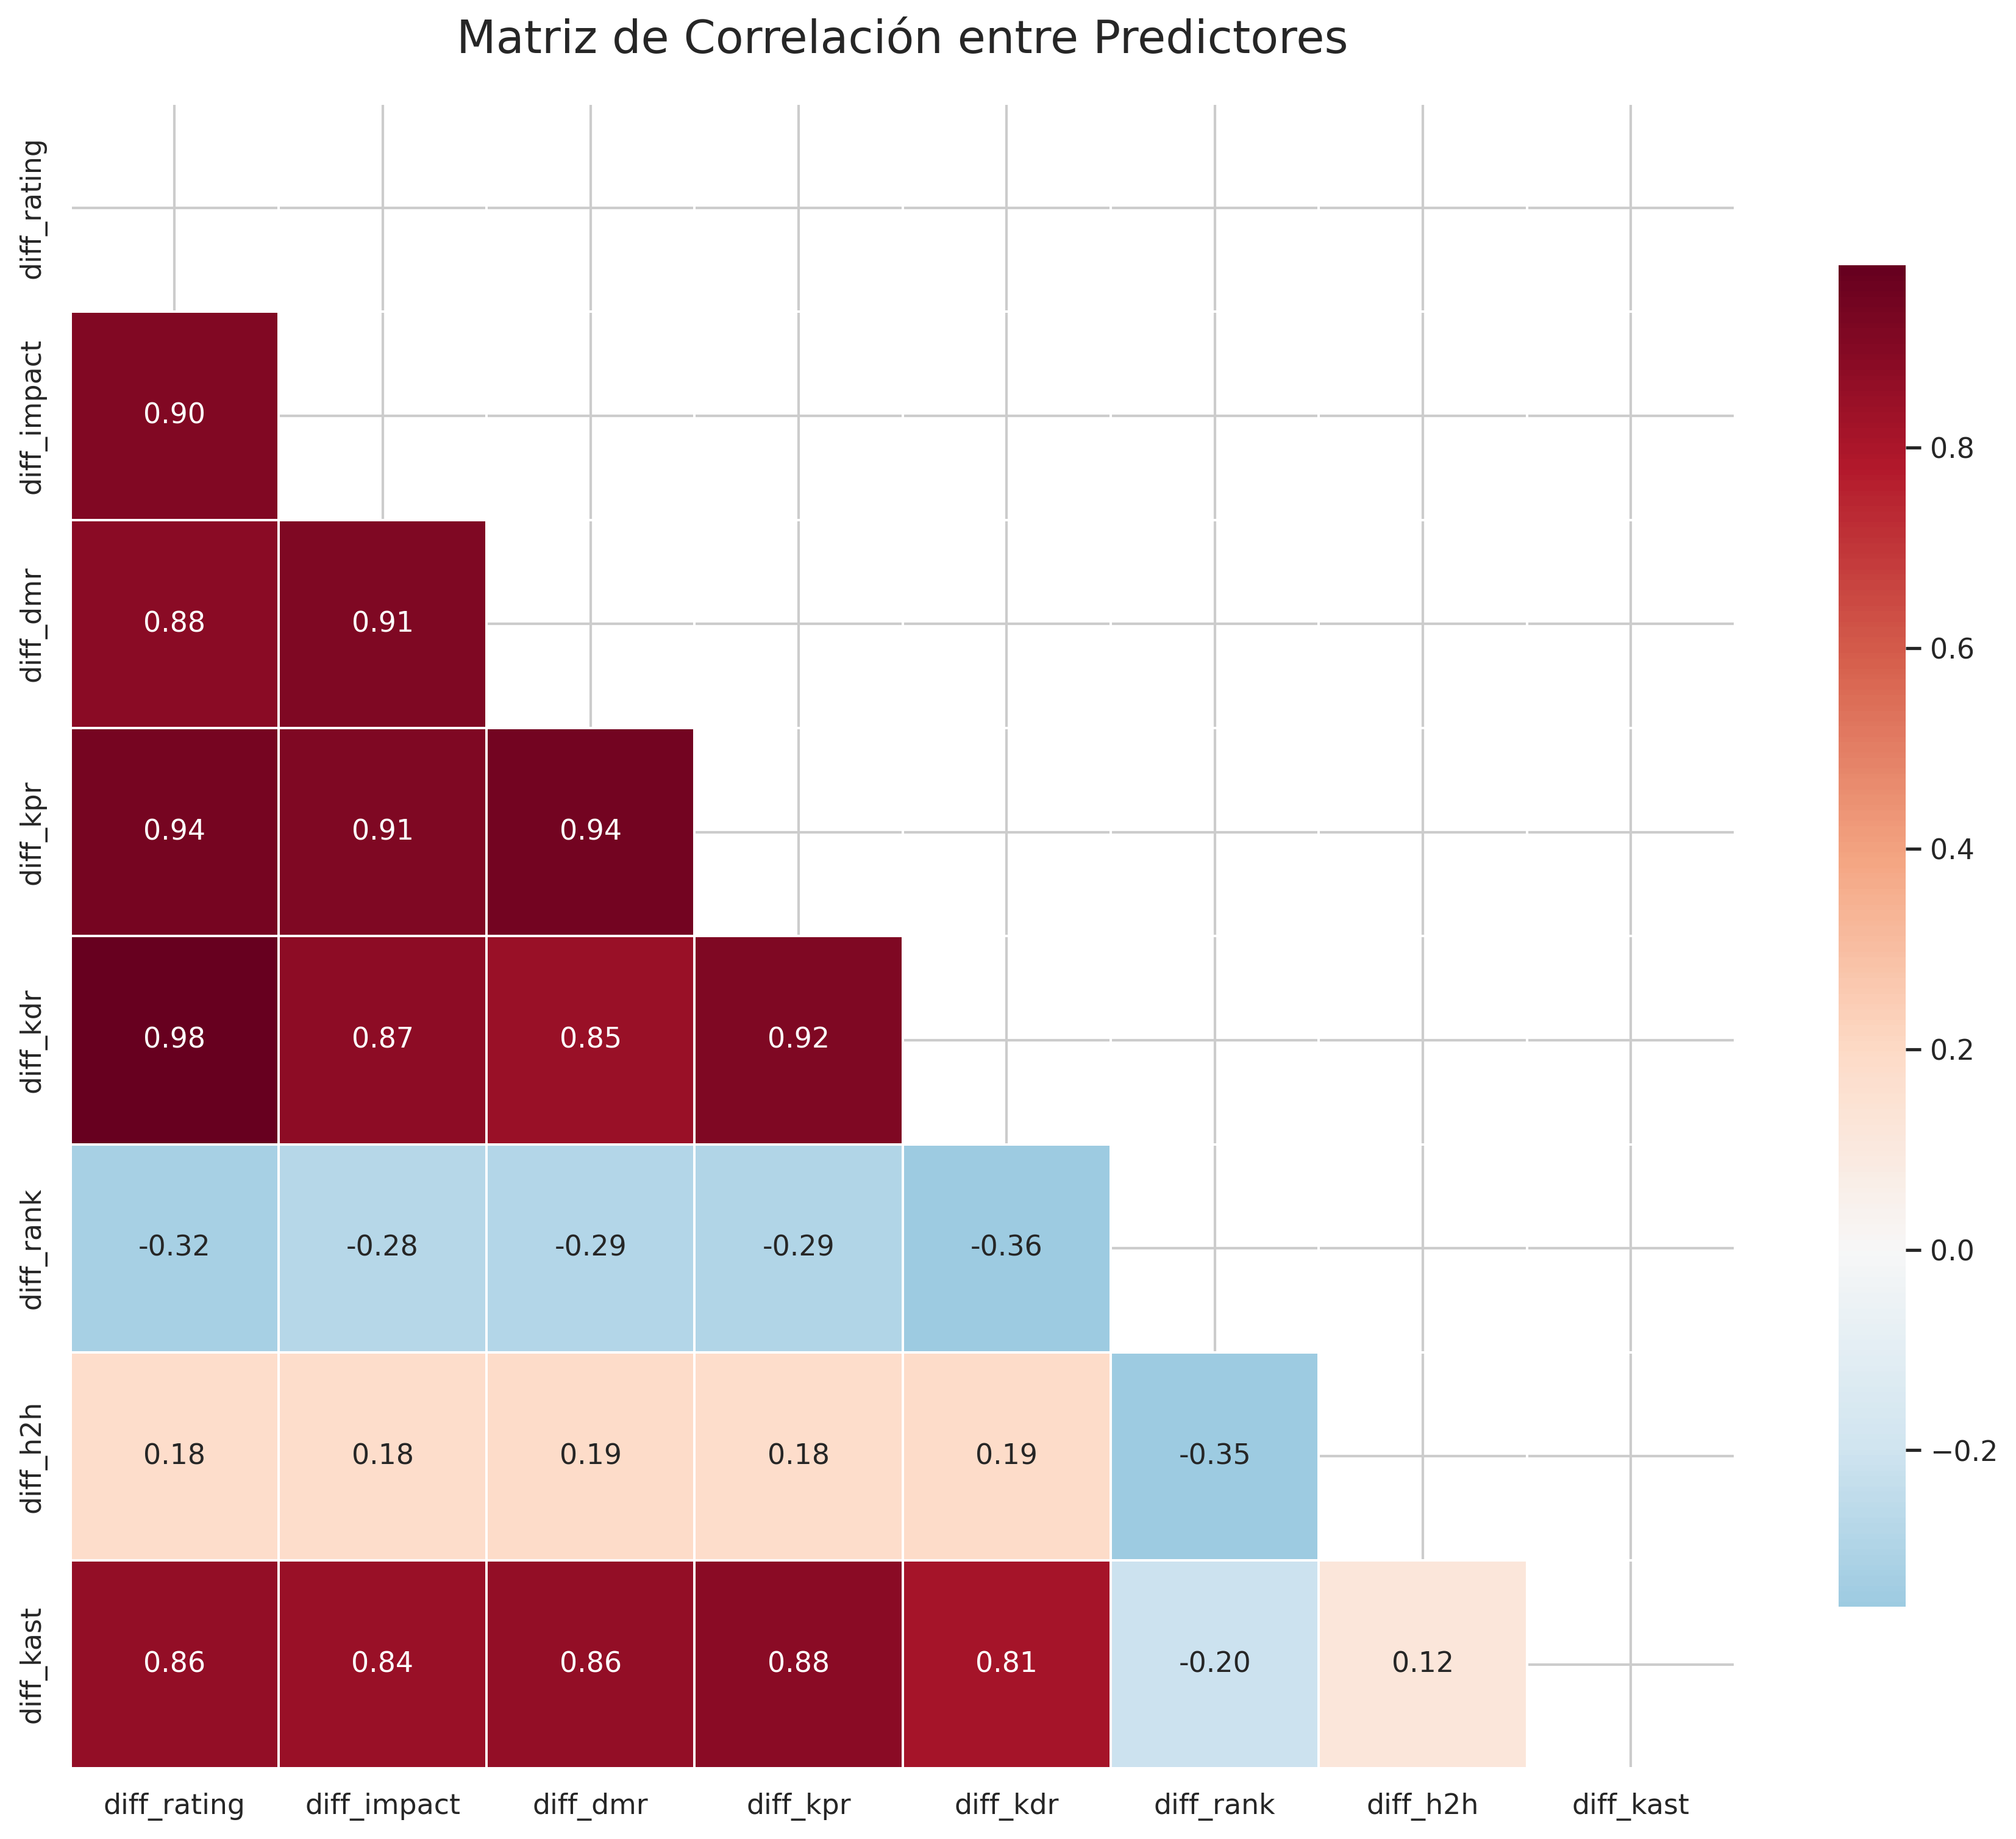
\includegraphics[width=\linewidth]{matriz_correlacion_completa.png}
    \caption{Matriz de Correlación: Descubriendo los motores de la victoria.}
    \label{fig:CorrFig}
\end{figure}

\section{DISEÑO METODOLÓGICO}
Para resolver nuestra duda, planteamos el problema mediante una \textbf{Regresión Logística Bayesiana Jerárquica}. Este enfoque permite no solo predecir el resultado, sino entender la estructura de incertidumbre detrás de cada variable competitiva.

\subsection{Definición de la Función de Verosimilitud (Likelihood)}
Dado que el resultado de un encuentro en el servidor es una variable binaria (victoria o derrota), se define el \textit{likelihood} mediante una distribución de \textbf{Bernoulli}:

\begin{equation}
    y_i \sim \text{Bernoulli}(p_i)
\end{equation}

Donde $p_i$ representa la probabilidad de éxito de un equipo en la partida $i$. Para relacionar esta probabilidad con el desempeño técnico, utilizamos la función de enlace \textit{logit}, que transforma el espacio lineal de los predictores al rango $[0, 1]$:

\begin{equation}
    \text{logit}(p_i) = \alpha_{map[i]} + \sum_{k=1}^{n} \beta_k X_{ki}
\end{equation}

Aquí, $X_{ki}$ representa variables como el \textit{Rating 2.0}, el \textit{Impacto} y el \textit{ADR}, mientras que $\alpha_{map[i]}$ actúa como un intercepto aleatorio que captura la variabilidad intrínseca de cada escenario de juego.

\subsection{Especificación de Priors y Argumentación}
En coherencia con el enfoque pedagógico de "honestidad estadística", se han seleccionado \textit{priors} que permiten al modelo aprender directamente de la evidencia de las partidas profesionales sin imponer sesgos restrictivos.

\begin{enumerate}
    \item \textbf{Coeficientes de Desempeño ($\beta_k \sim \text{Normal}(0, 5^2)$):} Se utilizan distribuciones normales débilmente informativas centradas en cero. Esto significa que el modelo comienza asumiendo que no sabe si variables como el \textit{Impacto} son positivas o negativas para la victoria, dejando que los datos dictaminen su verdadera influencia y magnitud.
    \item \textbf{Intercepto Jerárquico ($\alpha_{j} \sim \text{Normal}(\mu_\alpha, \sigma_\alpha^2)$):} Se reconoce que cada mapa de CS:GO posee una asimetría táctica única. Por ello, en lugar de un intercepto fijo, permitimos que cada mapa tenga su propia base probabilística, vinculada a una distribución global.
    \item \textbf{Hiperparámetros ($\sigma_\alpha \sim \text{HalfNormal}(2)$):} Para la variabilidad entre mapas, se utiliza una distribución \textit{Half-Normal}. Esto asegura que la desviación estándar sea siempre positiva y evita que el modelo sobreestime las diferencias extremas entre mapas con pocos datos.
\end{enumerate}

En la Figura \ref{fig:Priors} se puede apreciar cómo estas ideas sirven como el punto de partida probabilístico antes de que el proceso de simulación MCMC comience a integrar la evidencia del servidor.

\begin{figure}[h]
    \centering
    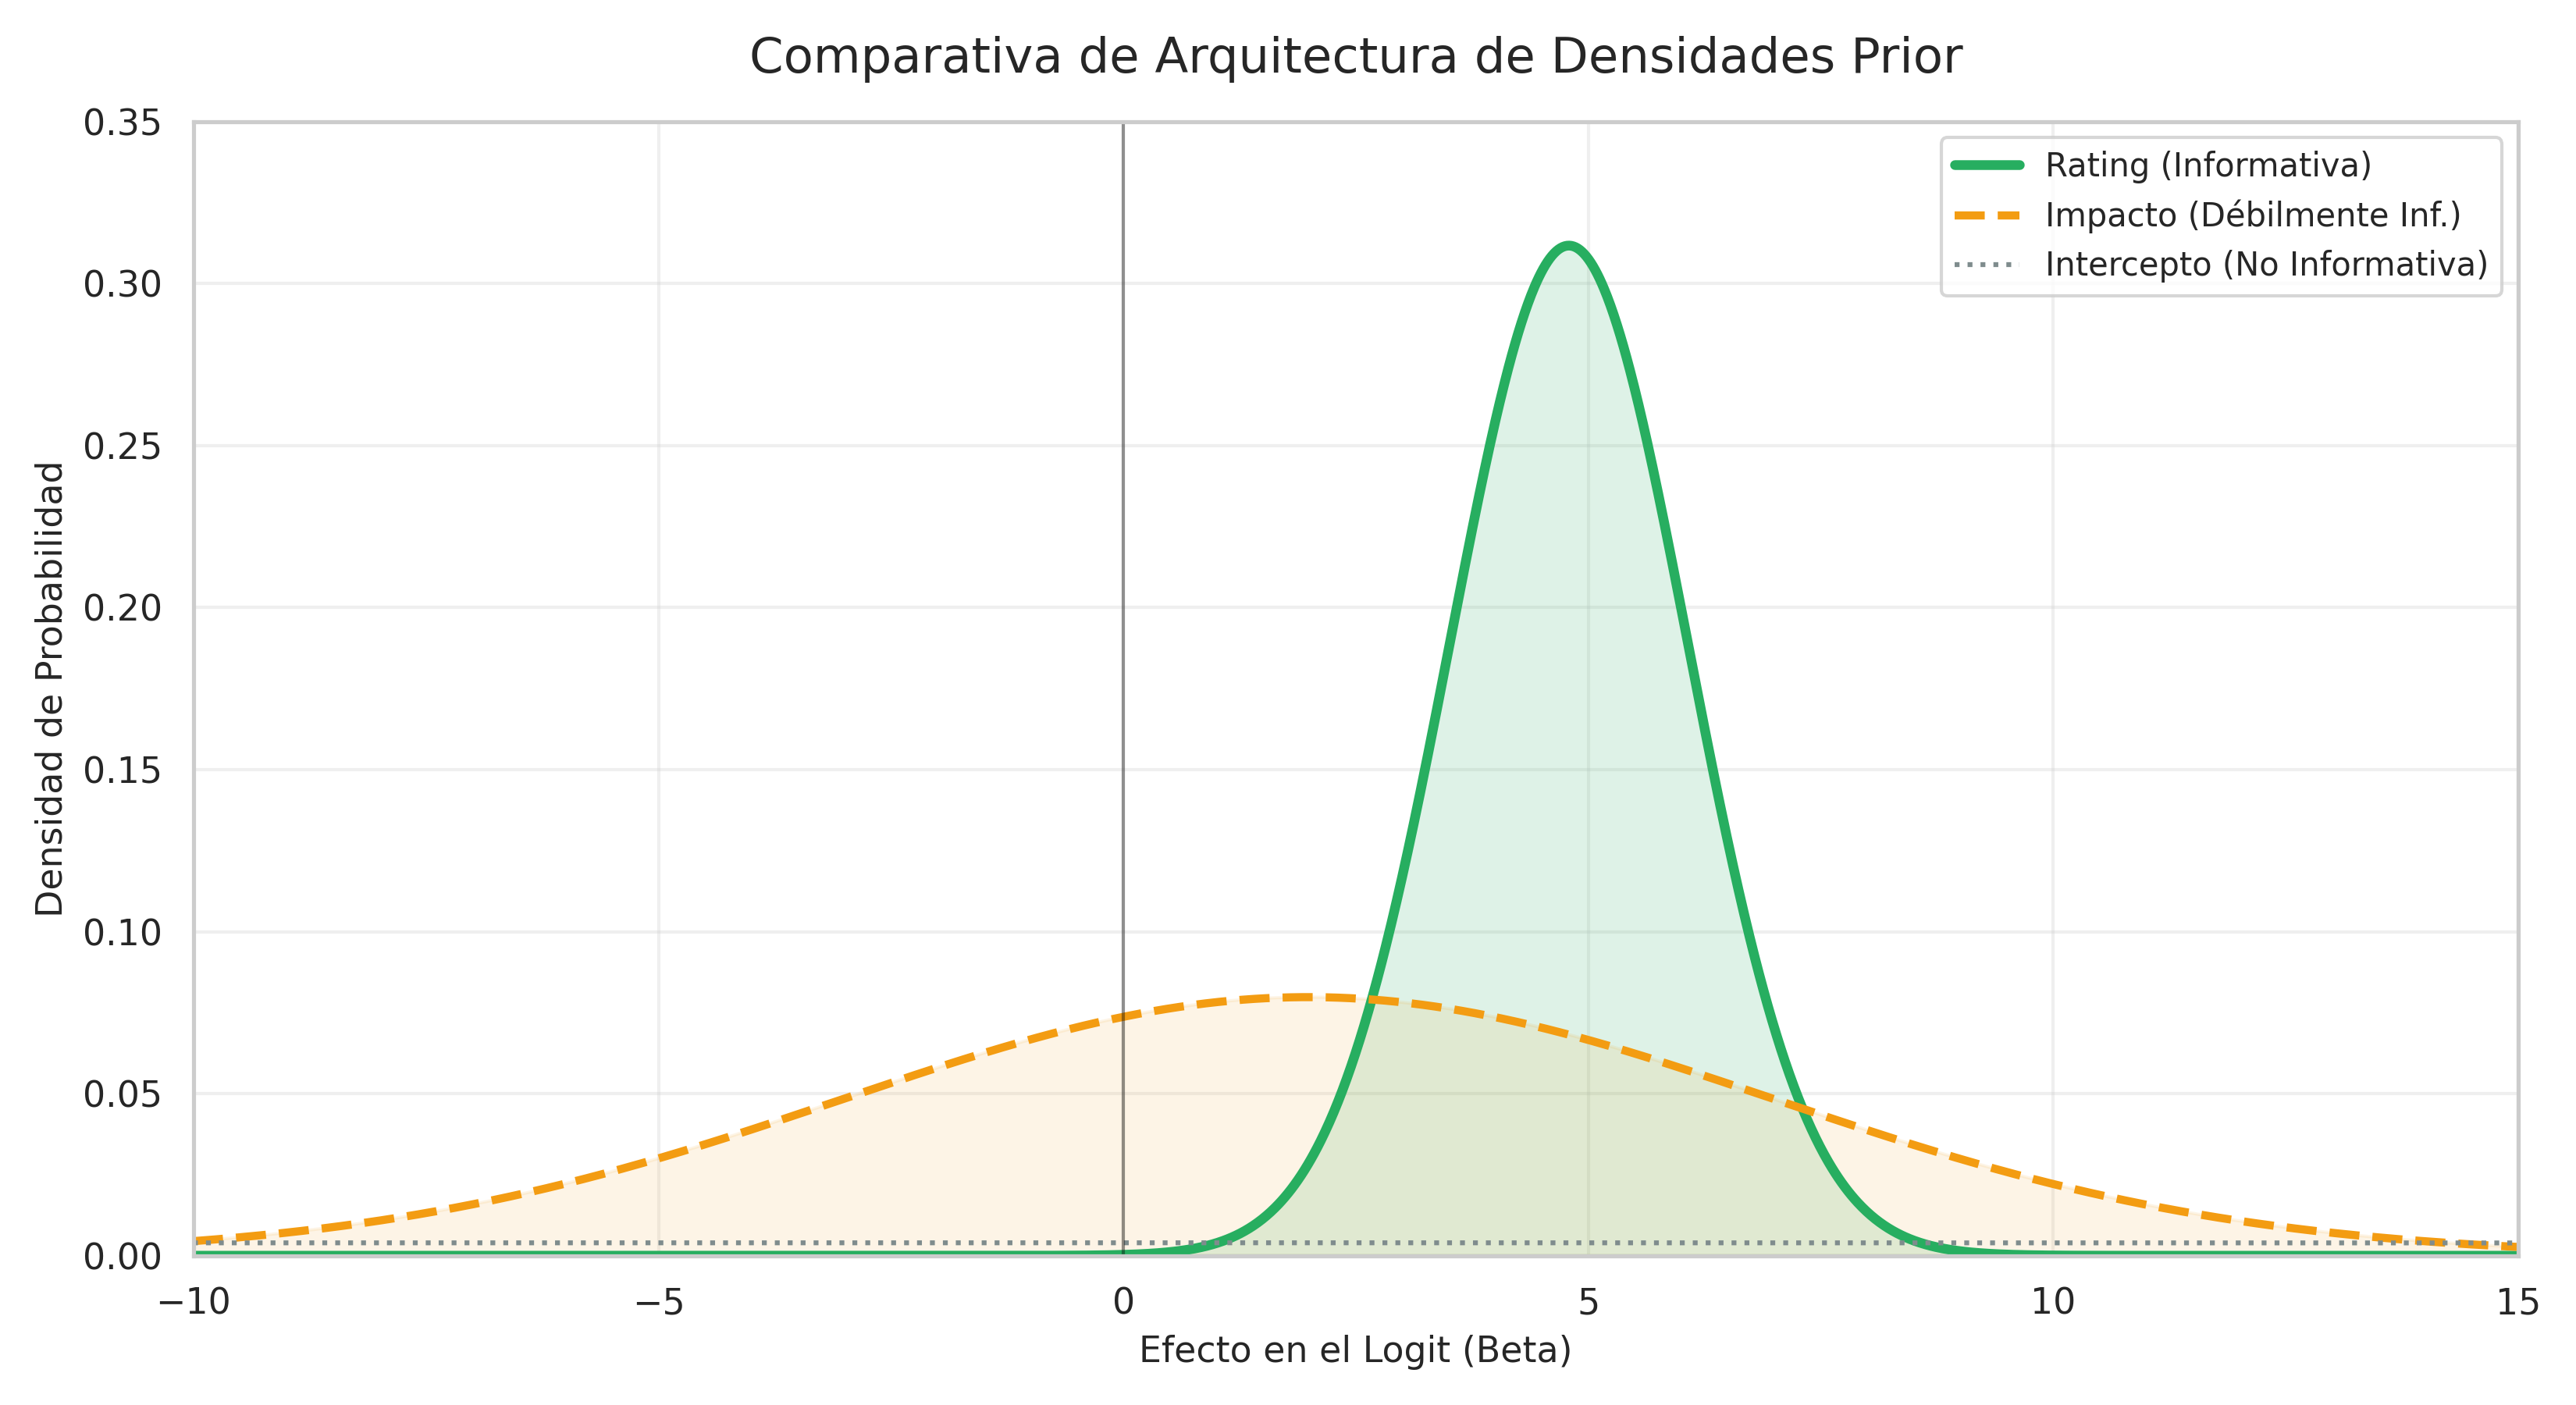
\includegraphics[width=\linewidth]{comparativa_priors.png}
    \caption{Comparativa de Priors: El punto de partida probabilístico.}
    \label{fig:Priors}
\end{figure}

\subsection{Estrategia de Evaluación}
Para saber si el modelo es confiable, se utilizan los \textbf{Chequeos Predictivos Posteriores (PPC)} para verificar que las simulaciones logren capturar la realidad del servidor, junto con el \textbf{HDI} para cuantificar la incertidumbre de las estimaciones. Un buen modelo es aquel que reconoce cuándo existe demasiada volatilidad como para asegurar un ganador.

\section{LIMITACIONES Y CONCLUSIONES}
Aunque se ha procedido con rigor, el modelo tiene sus límites, como no poder medir el estado de ánimo de los jugadores. Aún así, se llega a la conclusión de que la victoria no depende de un solo factor, sino de una combinación de variables donde el \textbf{Impacto Táctico} y el \textbf{Rating 2.0} se posicionan como las más influyentes. Además, se considera que el enfoque bayesiano es la mejor forma de dar predicciones ``honestas'' en un juego tan volátil e impredecible como el CS:GO.

\bibliographystyle{apalike}
\bibliography{bibliografia}

\end{document}
